\documentclass[edeposit,mixcasechap,tocnosub,noragright,centerchapter,fullpagesingle,12pt]{uiuc_csthesis21}

% Updated version of the ECE department's latex resources

% Use draftthesis for notes and date markings on every page.  Useful when you
%   have multiple copies floating around.
% Use offcenter for the extra .5 inch on the left side. Needed with fullpage and fancy.
% Use mixcasechap for compatibility with hyperref package, which does NOT like all caps default
% Use edeposit for the adviser/committee on the title page.
% Use tocnosub to suppress subsection and lower entries in the TOC.
% PhD candidates use "proquest" for the proquest abstract.

\makeatletter

\usepackage{setspace}  % Useful for single, 1.5, and double spacing
\usepackage{url}  % Useful for URLs
%\usepackage{hyperref}  % Another package useful for URLs

\usepackage{lscape}  % Useful for wide tables or figures.
% Following command definition is from Stack Exchange: https://tex.stackexchange.com/questions/278113/single-landscape-page-with-page-number-at-the-bottom 
% It adds *rotated* page numbers to the bottom of landscaped pages to meet the Graduate College standards (see page 7 here: https://grad.illinois.edu/files/pdfs/thesis-sample-chapter-straight-numbering.pdf)
\def\fillandplacepagenumber{
	\par
	\pagestyle{empty}
	\vbox to 0pt{\vss}
	\vfill
	\vbox to 0pt{
		\baselineskip 0pt
		\hbox to \linewidth{\hss}
		\baselineskip\footskip
		\hbox to \linewidth{\hfil\thepage\hfil}\vss
	}
}

% {{{ packages

\usepackage{blindtext}

% math
\usepackage{siunitx}
\usepackage{amsmath}
\usepackage{amsthm}
\usepackage{stmaryrd}
\usepackage{cases}
\usepackage{algorithm,algpseudocode}

% pretty links
\usepackage{xparse}
\usepackage{hyperref}
\usepackage[nameinlink]{cleveref}
\hypersetup{
    colorlinks=true,
    urlcolor=blue,
    citecolor=black,
    linkcolor=black
}

\usepackage{listings}
\usepackage{caption}
\usepackage{subcaption}

\usepackage{graphicx}

\usepackage[
    style=apa,
    backend=biber,
    style=numeric ]{biblatex}

% better environments
\usepackage[shortlabels]{enumitem}
\usepackage{booktabs}
\usepackage{caption}
\usepackage{multirow}

% graphics
\usepackage{tikz}
\usetikzlibrary{calc,arrows,automata,fit,positioning,shapes,chains, arrows.meta, chains, scopes,quotes, positioning}

% fancier font
\usepackage[sc]{mathpazo}
% better typography
\usepackage[activate={true,nocompatibility}, % activate protrusion and font expansion
            final,              % enable microtype, use draft to disable
            tracking=true,
            kerning=true,       % optimise interactions between characters
            spacing=true,       % more uniform spacing between words
            factor=1100,        % more protrusion
            stretch=10,         % smaller values (default 20, 20) to avoid blurring
            shrink=10]{microtype}
\SetTracking{encoding={*}, shape=sc}{40}

% }}}

% {{{ formatting

% enable section numbering only for the first three header levels
\setcounter{secnumdepth}{2}

% caption format
% NOTE: set format=plain to remove caption indentation
\captionsetup{
    format=hang
}

% allow subsubsections in the TOC, if there are any
% NOTE: if you got to subsubsections, you probably have too many!
\setcounter{tocdepth}{\subsubsectiontocdepth}
\setcounter{secnumdepth}{\subsubsectionnumdepth}

% NOTE: if there are many levels of indentation int the TOC, making it flat
% might be a good option with the following options
% \KOMAoption{toc}{indenttextentries,flat}

% https://marketing.illinois.edu/visual-identity/color
\definecolor{IlliniOrange}{RGB}{255, 95, 5}
\definecolor{IlliniAltgeld}{RGB}{200, 65, 19}
\definecolor{IlliniBlue}{RGB}{19, 41, 75}

\definecolor{IlliniAlmaMater}{RGB}{30, 56, 119}
\definecolor{IlliniIndustrialBlue}{RGB}{29, 88, 167}
\definecolor{IlliniArchesBlue}{RGB}{0, 159, 212}
\definecolor{IlliniCloud}{RGB}{248, 250, 252}
\definecolor{IlliniHeritageOrange}{RGB}{245, 130, 30}

% }}}

% {{{ commands

\NewDocumentCommand \dx { O{x} } {\,\mathrm{d} #1}
\NewDocumentCommand \vect { m } { \mathbold{#1} }
\NewDocumentCommand \od { m m } { \dfrac{\mathrm{d} #1}{\mathrm{d} #2} }
\NewDocumentCommand \pd { m m } { \dfrac{\partial #1}{\partial #2} }

% jump notation
\NewDocumentCommand \jump { sm } {
    \IfBooleanTF#1
    {\left\llbracket #2 \right\rrbracket}
    {\llbracket #2 \rrbracket}
}
% average notation
\NewDocumentCommand \avg { sm } {
    \IfBooleanTF#1
    {\left\langle #2 \right\rangle}
    {\langle #2 \rangle}
}
% inner product
\NewDocumentCommand \ip { m } { \avg{ #1 } }

\DeclareMathOperator{\tr}{tr}
\DeclareMathOperator{\sech}{sech}
\DeclareMathOperator{\argmin}{\operatorname{arg}\,\operatorname{min}}

% }}}

% {{{ environments

\NewDocumentCommand \newtheoremin { m m m } {
    \newtheorem{#1}{#2}
    \numberwithin{#1}{#3}
}
\newtheoremin{example}{Example}{section}
\newtheoremin{remark}{Remark}{section}
\newtheoremin{definition}{Definition}{section}
\newtheoremin{proposition}{Proposition}{section}
\newtheoremin{lemma}{Lemma}{section}
\newtheoremin{theorem}{Theorem}{section}

% }}}


\title{Emulation-Based Security Measurement with Applications in Avionics, Redaction, and Industrial Control}
\author{Maxwell Bland}
\department{Computer Science}

\schools{
B. S., University of Califonia, San Diego, 2018 \\
M. S., University of Califonia, San Diego, 2019 \\
}

\phdthesis
\advisor{Kirill Levchenko}
\degreeyear{2023}

\committee{
Professor Kirill Levchenko, Chair and Director of Research \\
Professor Adam Bates \\
Professor Aaron Schulman \\
Professor Gang Wang
}


\begin{document}

\maketitle

\parindent 1em%

\frontmatter

\begin{abstract}
The saftey of critical systems and data is of paramount importance to society.
Attacks on these systems can have catastrophic consequences, and the security of these systems is often difficult to measure.
Existing methods often involve access to ground-truth information, which is not always available.
In this dissertation, we explore the use of emulation to measure the security of systems in the absence of ground-truth information.

Complex system emulations often require sophisticated approaches to digital forensics and tactics for navigating undecidability resulting from uncertainty of the system's state.
To address these challenges, we present intelligent guess and check strategies for deducing hidden information in symbol-stripped binary firmware.
Our core technical contributions are (1) the first abstract interpretation based firmware rehosting system, used to generate emulations of embedded systems.
(2) A novel system for the analysis and recovery of glyph positioning information in PDF documents.
This system was used to recover redacted text information where the characters were removed in hundreds of sensitive documents.
(3) A logic-based intermediate representation and framework for the extraction of lifted function summaries from binary firmware.
This framework makes existing verification and synthesis techniques applicable to real-world systems by translating implemented code to mathematical models.
Where appropriate, we justify our strategies through discussions of correctness, precision, and generalizability.
Our results are never theoretical: we apply them to pre-existing, empirically validatable domain rather than models: among others, we study the Communication Management Unit used in Boeing 737 Aircraft, historically important redacted documents, and a programmable logic controller operating a Tennessee Eastman chemical plant reactor pressure valve.
\end{abstract}


\chapter*{Acknowledgments}

I would like to thank my advisor, Kirill Levchenko, for pushing me to standards and achievement few attain and for maintaining his support throughout the Ph.D. process.
Thank you to my committee members, Adam Bates, Aaron Schulman, and Gang Wang, for their support and guidance throughout the Ph.D., before, and in the completion of this disseration.

Thank you to Abraham Clements, Gabriela Ciocarlie, and Richard Kennell with CyManII for their support, advice, feedback, particularly in relation to the InteGreat system.
Additionally, I thank my collaborators Anthea Chen, Anushya Iyer, Stephen Checkoway, Stefan Savage, Joshua Mason, YiFei Zhu, Evan Johnson, Mingjia Huo, Stewart Grant, Alex Snoeren, Anil Yelam, and Nishant Bhaskar for their support and efforts throughout our papers together, though the subjects are not all approached in this thesis.
I also thank the University of Illinois, National Science Foundation, and CyManII for funding my research and efforts as a graduate student.

Additional thanks are in order for my labmates Tzu-Bin Yan, Margie Ruffin, Michael Chen, Megan Culler, Jonatas Marques, and many others at the Coordinated Science Laboratory who have provided support and friendship throughout my time at the University of Illinois, including Andrew Miller, Nikita Borisov, Michael Bailey, Deepak Kumar, Zane Ma, Paul Murley, Kyo Kim, and Joshua Reynolds.
I would also like to thank my friends in the Urbana-Champaign community, including Kevin Langowski, Alex Rogers and the Ship of Fools, the Rose Bowl, Waluigi's Mansion, the Spice Rack, and other basements unnamed who supported my harsh noise wall and other musical experiments.

Finally, thank you to Annika Sornson, whose love made me realize not all systems need to be broken: unfortunately, it was too late for the redactions, airplanes, and others.
Thank you as well to her parents for their support and friendship.
Finally, thank you to my parents and step-parents for their love and sacrifices.
Everyone mentioned above is impossible to emulate.



\begin{dedication}``For it is at the very moment when philosophy attempted for the first time to
	think rigorously the primacy of scientific knowledge that it decided to
	abjure precisely that aspect of thought which constituted the
	revolutionary character of scientific knowledge: its speculative
	import.'' \\
	--- \emph{Quentin Meillassoux}, After Finitude, p. 120.
\end{dedication}



% NOTE: recommended by the microtype docs to disable protrusion for the toc
\tableofcontents

% }}}

% {{{ main matter

\mainmatter

\chapter{Introduction}

Software systems, usually invisible to the end user, are ubiquitous in our daily lives.
They are used in a wide range of applications, from consumer electronics to critical infrastructure.
The security of these systems is paramount, as they are prevalent in our daily lives, however, analyzing these systems can be difficult as code and hardware may be opaque, meaning vulnerabilities may be known to specialized attackers that are not possible to measure automatically or easily.
Existing techniques often make strong assumptions about our understanding of the system, such as access to source code, non-symbol-stripped binaries, or mathematical models.

Conventional approaches rely on real-world testing or complex simulations, bug reports, high-level verification (formal methods), and manual analysis to find bugs and vulnerabilities.
There is nothing inherently wrong with any of these approaches, but they still have limitations due to complexity, cost, coverage, and effort involved, limiting these approaches to parties with sufficient resources to perform them.
And regardless of the approach taken to security, as with most problems, there remain unknown features of the system under analysis (or simply too many systems), making it potentially impossible to predict all future exploits.
In 2022, Mitre reported 34,553 CVE entries~\cite{mitre2022}, following a steady, monotonic increase from 2016.
Moreover, metrics for evaluating the complexity of source code are still fail to capture developer expectations~\cite{pantiuchina2018improving, feigenspan2011exploring, feitelson2023code}.
Even in the ``good'' case, where we have perfect ground truth for a system, algorithms struggle to make accurate judgements of general constructs in real systems, judgments necessary to determine systems' security.

The security of a system hinges on whether the flaws in the system are represented in an accessible medium whereby they are effectively identified and corrected, a hard problem as every measurement exists in a specific interpretive context~\cite{stolfo2011measuring}.
Each paradigm for securing a system, e.g. a provably correct decision system, implicitly determines which flaws are considered or prevented and which are overlooked.
Ultimately a variety of approaches are necessary to secure a system and all of them, in principle, make some statement about the observable behavior of the system during operation.
Security is a veritable symbolic arms race towards better representations and emulations, as evidenced by recent works~\cite{shoshitaishvili2016sok, arp2022and, chen2022metaemu}, including works from this dissertation~\cite{johnson2021jetset, bland2023story, bland2023integreat}.
In this dissertation, we present several novel approaches to the representation and emulation of complex, opaque software systems, broadly applicable and empirically capable of identifying flaws in and exploits for real-world avionic, PDF document redaction, and industrial control systems.

\paragraph{Terminology}
This dissertation focuses on single, specific concept of \emph{emulation} as applied to systems.
We define emulation as the process of executing a model of the system where at least one component is not represented during simulation on some kind of host computer~\cite{marwedel2021embedded}.
Perfect \emph{simulation}, on the other hand, involves modeling the entire underlying state of the target.
Implied in this definition is the fact that emulation embraces speculation, non-exact representation, and a lack of ground truth for the system being analyzed, making it more broadly applicable than simulation for complex systems.
Emulations, simulations, and the systems in question are subjects of \emph{dynamic analysis}, which attempts to run the program and analyze its execution, introduced by Ball in 1999~\cite{ball1999concept}.
Dynamic analysis is contrasted with \emph{static analysis}, which attempts to analyze the program without running it and also attempts to make statements about the dynamic behavior of the system~\cite{chess2004static}.
In either case, the purpose of these analyses is typically to enforce some requirement (also called property or specification), to represent the desired behaviors of the system, such as safety, stability, or temporal constraints, falling into the subdomain of formal methods~\cite{woodcock2009formal, leeb2005proving}.
More generally though, emulations can be used to imperfectly replace the system in question, aiding in processes falling outside the purview of verification, such as binary exploit development, information leak detection, and behavioral prediction~\cite{huang2014software, le2018micro, landsiedel2005accurate}.

Within the broad areas of emulation and simulation, this dissertation focuses on three strategies or techniques: \emph{rehosting}, \emph{dictionary attacks}, and \emph{lifting}.

\paragraph{Rehosting}
Rehosting is the process of bootstrapping a system so that it can be emulated in a different context, typically a laptop computer instead of the original embedded system, e.g. a programmable logic controller.
This encounters the particular challenge of modeling or reimplementing subsystems or subcomponents that are not present in the new context, such as hardware devices.
If a ground truth reference for the subsystem's behavior is available, then this can be used to bootstrap a simulation of it (or sometimes a connection to the subsystem itself) in the new context, but this is not always the case.
In cases where a ground truth reference is not available, the behavior of the subsystem must be inferred from residual information recoverable from the system, such as binary code for interacting with the subsystem.

\paragraph{Dictionary Attacks}
A brute force approach to emulation that attempts to perform a universal quantification of the possible true behaviors of the system and then use some checking or verification mechanism to isolate the correct behavior.
In many cases it is possible to extract a function from a program, and evaluate it in isolation of the rest of the system for all possible given inputs, recovering all possible outputs.
We also classify fuzzing, the process of mutating inputs to a system to find unexpected behaviors, as a form of dictionary attack.
This can precisely determine what the system is capable of in circumstances where a specific function can be isolated, the number of possible inputs is constrained, and a precise verification mechanism is available.

\paragraph{Lifting}
Lifting is the process of translating the representation of a system into a different symbolic domain which is easier to reason about.
The result of lifting is an intermediate representation or extracted model of the system.
An example of this is a translation from binary code to mathematical statements which can be emulated outside of the complex context of software, e.g. one with hardware device models.
While this can potentially miss the validation of critical components, careful lifting can also avoid the necessity of reasoning about unknowns in the system.

\paragraph{Challenges}
Rehosting, dictionary attacks, and lifting each have their own challenges in generalization, scalability, and completeness respectively~\cite{wright2021challenges, delaune2004theory, reps2006intermediate}.
Significant progress continues to be made in addressing these challenges in order to apply each of these techniques to practical problems, and approaches to emulation are often mixed in order to acheive effective results~\cite{p2im2020, clementshalucinator, li2018fuzzing, zheng2019firm, yun2018qsym, borzacchiello2021fuzzolic}.
However, each of these strategies presents a perspective on the problem of evaluating a system in the absence of a complete model, and so all recent work shares a common goal of determining knowable and unknowable features or flaws in a system.

\paragraph{Dissertation Topics}
Whereas verification enforces a specific representation of a system through mathematical proof, emulation strives to develop a useful clone of the system for another context.
More recent data-driven verification approaches bridge this gap but do not approach the subject of emulation and how it affects modeling.
This dissertation does not provide a framework for completing all incomplete system models but does make progress the above common goal by introducing theories on or strategies for the emulation of complex systems.
One shared theme is the use of subtle information present in things which are distinctly not the system in order to emulate the system.
As a result, our strategies are particularly useful for real-world systems of which only some qualities are known or accessible.
Thus, we are also able to provide evidence of our theories' effectiveness in practice and provide insight into the absolute limits of emulation.

Correct emulation also implies avoidance towards making unjustified assumptions about possible states or accurate respresentations of the system under analysis.
A complete description of the problem acknowledges mathematics is incapable of conferring a priori existence upon its subject and adopts conceptual or empirical strategies into the execution and analysis of unknown system features.
In the description of these strategies for emulation, we will find the application of guesswork is unavoidable, and that these guesses must later be checked and verified against the system itself.
Luck and probability play an integral role in the application of emulations and the proper use of emulation often requires the joint application of uncertainty and sensitivity analysis, but we will not limit ourselves to analyzing emulations in terms of axiomatics or quantification via a unifying theory.
Instead, in this dissertation, we discuss the symbolic representations that exist prior to analysis and effects of interpretive frameworks on the generation of emulations from the context of:

\begin{enumerate}
	\item the synthesis of hardware models from software information~\cite{johnson2021jetset} (Chapter~\ref{chap:rehost}),
	\item the determination of text content after it is removed (redacted) from PDFs~\cite{bland2023story} (Chapter~\ref{chap:info}), and,
	\item the use of logic-based intermediate representations for lifting between symbolic domains~\cite{bland2023integreat} (Chapter~\ref{chap:integreat}).
\end{enumerate}

With exceptions for the implementation of a taint-tracking based symbolic execution system in QEMU and some ideas relating to symbolic search strategies (Chapter~\ref{chap:rehost}), the information leak quantification for specific redaction dictionaries (Chapter~\ref{chap:info}), as well as the analysis of the quadcopter stabilization algorithm (Chapter~\ref{chap:integreat}), which were implemented jointly with coauthors, the works presented in this dissertation are the author's own with dialectic support from coauthors.

We next provide a more detailed introduction to each of the above topic areas, followed by a summary of contributions and impacts.

\section{Targeted Firmware Rehosting for Embedded Systems}

The possession of a physical copy of a critical system for analysis is often difficult.
Additionally, it is valuable to attain an emulated copy of these systems for the purposes of precise, invasive analysis without binary rewriting.
Implementing an emulation of a system's hardware devices is labor intensive, therefore, automated methods for generating emulated, rehosted copies of systems are valuable.

In this dissertation, we discuss the possibility of generating emulations of hardware from information present in firmware alone, with the first strategy being the symbolic analysis of firmware interactions with hardware devices.
By collecting the constraints software places on the function of hardware during interaction with hardware peripherals, it is possible to synthesize a model of the hardware device.
We show the limitations and challenges involved in this analysis and find that in many cases it is possible to use this partial constraint information to generate a useful emulation of associated hardware.
In solving this challnge, we introduce one of the first fuzzing systems targeted at arbitrary QEMU system simulations, and several tactics for dealing with undecidable problems related to symbol-stripped, binary program analysis.
We applied this system to more than ten firmware images, but we focus on one in particular, the Communication Management Unit of a Boeing 737, and other aircraft, responsible for managing a large part of the communication of key Line Replacable Units (LRUs) in the aircraft, including the Flight Management Computer.
Our emulated hardware not only allowed us to develop an effective rootkit and local code execution attack on the CMU, but also identify three remote messages capable of powering down the machine, creating a denial-of-service attack.\footnote{Due to their sensitivity, the specifics of these exploits are not given explicit detail.}

In the preliminary section of this dissertation, we introduce the notion of abstract interpretation as a method of reasoning about symbols inside of algorithms.
This method was implied in the form of symbolic execution within the Jetset system~\cite{johnson2021jetset}, where it was able to rehost all the devices targeted by an ``equivalent'' fuzzing approach~\cite{p2im2020}, as well as and SEL Feeder Protection relay controlling breaker switches in electrical substations~\cite{feederprotection}, the aforementioned CMU-900~\cite{cmudevice}, and various SoCs (Raspberry Pi 2 and BeagleBoard-xM)~\cite{raspbpi, beagleboard}.
The rehosted emulations can be subject to several forms of potentially destructive dynamic analysis routines that would be impossible on the physical device, such as fuzzing, which may ``brick'' the device in question.
The use of symbolic execution for rehosting-related tasks has now been adopted and integrated into several additional research works in top venues to rehost a variety of systems~\cite{zhou2022your, chen2022metaemu, hernandez2022firmwire, sun2022spenny}.
A complete explication of the challenges and techniques involved in rehosting is beyond the scope of this disseration and we refer interested readers to~\cite{wright2021challenges}.

\section{Glyph Positions Break PDF Text Redaction}

The analyis of embedded systems is just one application of emulation---emulation of software systems can also play a vital role in the analysis of information leaks.
By extracting and emulating the glyph positioning behavior of popular PDF document creation software, it is in fact possible to generate precise fingerprints for the layout of text on a page.
It turns out that this layout contains sub-pixel error-correction information which leaks a large amount of information about any text redactions where characters are removed the document's digital representation.

To emulate these different PDF creation software stacks and break redactions, we developed a novel framework Edact-Ray~\cite{bland2023story} which attempts universal quantification over potential redacted texts in emulation to identify the input which produced the PDF document under analysis.
The system also includes scripts which are capable of analyzing thousands of PDF documents and locating vulnerable redactions in these documents in bulk.
Using access to the RECAP court document system~\cite{recap}, we were also able to identify hundreds of non-excising redactions where the text was simply covered with a black box rather than being removed from the PDF, resulting in the discovery of confidential trade secrets for large corporations, the addresses of famous US celebrities, and salacious statements.
This has resulted in the notification of hundreds of lawyers involved and significant efforts to make redaction uniform across court systems.

We used the Edact-Ray system to break a number of historically relevant redactions otherwise thought to be secure.
These include redactions in documents from the Digital National Security Archives (DNSA)~\cite{dnsaSite}, and the US Court System~\cite{pacerSite}.
We also used the system to identify hundreds of broken redactions in Office of Inspector General (OIG)~\cite{oigReports} and Freedom of Information Act (FOIA) documents~\cite{govattic}.
Our findings resulted in the notification of more than 22 different US government agencies, national media recognition~\cite{wired} and extensive collaborations on working towards a solution to the problem of broken redactions.

\section{Lifting Continuous Control Equations from Binary Code}

The last topic addressed in this dissertation is a bottom-up approach to verification, a 
system for lifting discrete binary code algorithms to the continuous domain for simulation
in frameworks like Matlab Simulink~\cite{bland2023integreat, matlab}.
We consider the possibility of representing symbolic translation rules in a logic-based intermediate representation, where microarchitectural features are modeled deductively and complex statements about program semantics may be derived by nesting simpler statements.
Intermediate representations for the purposes of lifting (decompilation), translation, and emulation are an active area of research and are used by several high-powered offensive analysis tools such as angr and Ghidra, however, logic has not yet been used as a syntax for describing microarchitectural features in a decompiler~\cite{lattner2021mlir, quinlan2000rose, chen2022metaemu, eagle2020ghidra, kim2017testing, stanier2013intermediate}.

As a result, current intermediate representations for binary analysis suffer from several drawbacks related to nesting and translation.
They strive for a static representation of program semantics rather than one which must be dynamically evaluated, limiting their representational capacity for more complex semantic structures present in code.
This dissertation explores the possibility of using a logic-based intermediate representation to lift continuous control equations from the binary firmware of Cyber-Physical Systems~\cite{letichevsky2017cyber}.
We begin by representing and lifting simple microarchtectural semantics, such as the splitting of a floating point number split across registers 0 and 1 in the ARM architecture.
These rules are then nested into more complex deductive chains, such as the structure of common mathematical functions, through the use of statements in propositional logic over the theory of uninterpreted functions\footnote{Uninterpreted functions discard the computation under analysis and reduce it to a single symbol and list of input, output locations.}.
Once specified, these rules are combined with abstract interpretation, which identifies the specific relations between input and output locations, in order to translate logically-defined program slice boundaries in the system under analysis to relations and operations over uninterpreted functions.
When correctly performed, this method lifts implicit, abstract semantics from a binary firmware images, e.g. mathematical functions like cosine.

We implemented this approach in a tool called InteGreat and use the tool to extract functions from a Programmable Logic Controller (PLC) used to control the reactor pressure of a chemical plant, as well as the stabilization algorithm of a quad-copter and a single backpropagation step in an artificial neural network.
InteGreat does not just lift program slices to the continuous domain using the logical statements embedded in its intermediate representation: it then translates the lifted representation into a Matlab emulation of the system, allowing us to model precise destabilization attacks on the chemical plant and identify flaws in implementations and published versions of the quad-copter's stabilization algorithm.

\section{Summary of Contributions}

\section{Dissertation Structure}

\chapter{Preliminaries}
\label{chap:prelim}

Here, we introduce concepts, vocabulary terms, operations, and initial related work that is referenced throughout this disseration.
The theme of each of these subject areas is the representation of information, whether that information relates to the operation of binary code, the content of removed text, or a deduced interpretation of an existing system.

\section{Abstract Interpretation}

Under the traditional definition, \emph{abstract interpretation} is a method of approximating the behavior of a program using monotonic functions over ordered sets (typically lattices).
It is related to the emulation of a program in that it is intended to extract a model of the program's behavior without performing the exact computations involved.
However, abstract interpretation has become more of a general framework for defining relations between different domains, as the necessity of translation between dissimilar symbolic representations, e.g. in transpilers, has become more prevalent.

Arbitrarily, let $L$ and $L'$ be \emph{concrete} and \emph{abstract} ordered sets, repectively.\footnote{The ordering of higher or lower levels of abstraction themselves is a function over the mathematical structures being discussed.}
These sets are related to each-other by a total function, which maps elements in one set to another.
We define two functions, $\alpha$ and $\gamma$, which map elements of $L$ to $L'$ and vice versa, and are called the \emph{abstraction} function and \emph{concretization} function respectively.

Then, given ordered sets $L_{1}, L_{2}, L'_{1}, L'_{2}$, the concrete semantics $f$ is a monotonic function from $L_{1}$ to $L_{2}$, and a correct abstraction from $L$ to $L'$ is \emph{valid} if the abstract semantics $f'$ mapping $L'_{1}$ to $L'_{2}$ preserves the ordering in $f$ of $L_{1}$ to $L_{2}$.
In this definition the ordering operation on the sets is left undefined, and in the absence of a decidable set of mathematical qualities, e.g. many nontrivial computer programs, so standard implementations of abstract interpretation on program execution operate by mapping between a concrete execution trace in registers and memory and the theory of bitvectors, rather than the highly abstract semantics used by programs' users and authors.

\subsection{Symbolic Execution}

This specific form of abstract interpretation is called \emph{symbolic execution}, and is a method of program analysis that operates by tracking the values of variables in a program as symbolic expressions, rather than concrete values.
For example, in standard execution the statement $(x > 5) ?\ y + 1 : x + 1$ would be concretely evaluated to 4 if $x = 3$, however, a standard symbolic execution, the system will record the pair $(x<=5; x=x+1),(x>5;x=y+1)$ into a symbolic state, representing the two possible execution paths.

Symbolic execution is a powerful tool for program analysis, but it is not without its limitations.
The core challenge is the \emph{path explosion} problem, where the number of possible execution paths grows exponentially with the number of branches in the program.
This can be limited through \emph{loop invariant} analysis, where the system attempts to identify the invariants of a loop and only execute the loop a finite number of times, a \emph{search strategy}, which determines which execution paths to explore from the exponential number possible, or a number of other deductive techniques.
Closely related is the challenge of \emph{memory aliasing}, which occurs when the system is unable to determine whether two pointers point to the same memory location, as the values of each pointer are treated as symbolic expressions over the theory of bitvectors rather than concrete values.
Additionally, there is the \emph{environmental modeling} problem, where symbolic execution is unsound due to missing context, typically because the specific execution behavior of the hardware is not present, e.g. interrupts or highly-specific microarchitectural features.

\subsection{Lifting}

We contrast abstract interpretation with the notion of \emph{lifting}, a borrowed term concept from category theory, where given a structure-preserving map from one mathematical structure to another of the same type (a morphism), $f: X \rightarrow Y$,  and another $g: Z \rightarrow Y$, a lifting of $f$ to $Z$ is a morphism $h: X \rightarrow Z$ such that $f = g \circ h$, or more simply, a function that points to another representation that \emph{may} more closely resemble the structure $Y$ but also has a morphism to $Y$ (Fig.~\ref{fig:lift}).

\begin{figure}[h]
\centering
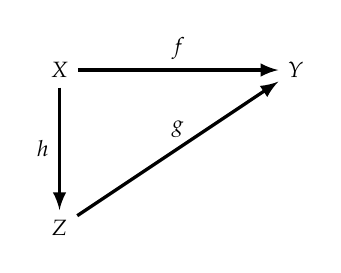
\begin{tikzpicture}[
  >=latex,
  every edge/.style={draw, very thick},
  every node/.style={font=\footnotesize},
  lift/.style={draw=none, fill=none}
  ]
  \node (X) at (0,0) {$X$};
  \node (Y) at (3,0) {$Y$};
  \node (Z) at (0,-2) {$Z$};
  \draw[->] (X) edge node[above] {$f$} (Y);
  \draw[->] (Z) edge node[above] {$g$} (Y);
  \draw[->] (X) edge node[left] {$h$} (Z);
\end{tikzpicture}
\caption{Lifting $f$ to $Z$}
\label{fig:lift}
\end{figure}

When applied to code, lifting typically refers to exposing the semantic structure of the binary to a higher level of abstraction.
However, as the mathematical definition suggests, lifting may also refer to a \emph{different} structure with the same morphism to the ``true'' structure.
Note that lifting is a form of \emph{translation}, but the new structure exists over a different domain.
For example, machine code may be lifted to a symbolic representation that represents a call-graph, or it may be lifted to a higher-level language, e.g. C, but it would be translation rather than lifting if the code was made into an equivalent, different machine code, e.g. ARM to x86.

Standard forms of lifting include translating a program into a form of graph representing latent relationships in the program, in order to simplify algorithms for reasoning about the program's structure.
For example, a program may be translated into a \emph{control flow graph} (CFG), where each node represents a basic block of code and each edge represents a possible transition between blocks.
Figure~\ref{fig:cfg} shows an example of lifting a CFG from a simple machine code program.

\begin{figure}[h]
\centering
\begin{tikzpicture}[
  >=latex
]
% split the picture into two halves. on the left have the disassembly and on the right the CFG
% disassembly with a simple branch
\node (disassembly) at (0,0) {
\begin{tabular}{ll}
\texttt{0x0} & \texttt{mov eax, 0x0} \\
\texttt{0x5} & \texttt{mov ebx, 0x1} \\
\texttt{0xa} & \texttt{cmp eax, ebx} \\
\texttt{0xc} & \texttt{jne 0x15} \\
\texttt{0xe} & \texttt{mov eax, 0x1} \\
\texttt{0x13} & \texttt{jmp 0x1a} \\
\texttt{0x15} & \texttt{mov eax, 0x0} \\
\texttt{0x1a} & \texttt{ret}
\end{tabular}
};
% CFG
\node (cfg) at (6,0) {
\begin{tikzpicture}[
  >=latex,
  every edge/.style={draw, very thick},
  every node/.style={font=\footnotesize},
  lift/.style={draw=none, fill=none},
  block/.style={draw, rectangle, minimum height=0.5cm, minimum width=0.5cm}
  ]
  \node[block] (0) at (-3,-2) {\texttt{0x0}};
  \node[block] (5) at (-1.5,-2) {\texttt{0x5}};
  \node[block] (a) at (0,-2) {\texttt{0xa}};
  \node[block] (c) at (0,-3) {\texttt{0xc}};
  \node[block] (e) at (0,-4) {\texttt{0xe}};
  \node[block] (13) at (0,-5) {\texttt{0x13}};
  \node[block] (15) at (-1.5,-6) {\texttt{0x15}};
  \node[block] (1a) at (0,-6) {\texttt{0x1a}};
  \draw[->] (0) edge (5);
  \draw[->] (5) edge (a);
  \draw[->] (a) edge (c);
  \draw[->] (c) edge (e);
  \draw[->] (e) edge (13);
  \draw[->] (15) edge (1a);
  \draw[->] (c) edge[bend right=30] (15);
  \draw[->] (13) edge (1a);
\end{tikzpicture}
};
% draw an arrow between the two halves
\draw[->, very thick] (disassembly) edge (cfg);
\end{tikzpicture}
\caption{Lifting a CFG from machine code}
\label{fig:cfg}
\end{figure}

\emph{Program slicing} is a form of lifting which transforms a program specification into \emph{slices}, sets of statements affecting sets of values in the program's state at some points of interest.
More generally, they may also refer to arbitrary subsets of the program's statements.
The determination of the slices is typically referred to as a \emph{slice criterion}.
Symbolic execution can be used to determine a given slice by exploring all paths through a program and thus the statements which affect the value of a variable of interest.

\subsection{Intermediate Representations}

The term \emph{intermediate representation} (IR) refers to a representation of a program that is used as an intermediate step a translation process, typically for a compiler.
The IR is typically designed to be easy to translate to and from the source and target languages, and to be easy to reason about.
Referring to Fig.~\ref{fig:lift}, in lifting the IR is the structure $Z$ used to translate between $X$ and $Y$.
The critical form of IR for use in symbolic execution and abstract interpretation more generally are abstract syntax trees (ASTs).
ASTs are a form of IR that represent the syntactic structure of a program as a tree, where each node represents a syntactic construct and each edge represents a relationship between constructs.
For example, the AST for the expression \texttt{a + b * c} is shown in Fig.~\ref{fig:ast}.

\begin{figure}[h]
\centering
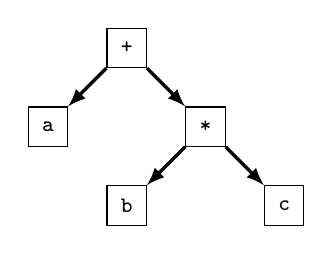
\begin{tikzpicture}[
  >=latex,
  every edge/.style={draw, very thick},
  every node/.style={font=\footnotesize},
  lift/.style={draw=none, fill=none},
  block/.style={draw, rectangle, minimum height=0.5cm, minimum width=0.5cm}
  ]
  \node[block] (plus) at (0,0) {\texttt{+}};
  \node[block] (a) at (-1,-1) {\texttt{a}};
  \node[block] (times) at (1,-1) {\texttt{*}};
  \node[block] (b) at (0,-2) {\texttt{b}};
  \node[block] (c) at (2,-2) {\texttt{c}};
  \draw[->] (plus) edge (a);
  \draw[->] (plus) edge (times);
  \draw[->] (times) edge (b);
  \draw[->] (times) edge (c);
\end{tikzpicture}
\caption{AST for \texttt{a + b * c}}
\label{fig:ast}
\end{figure}

% relate IRs to Hoare Logic. Is Hoare Logic an IR?
ASTs may be used in conjunction with \emph{Hoare logic} to reason about programs.
Hoare logic is a formal system for reasoning about the correctness of programs.
It is based on the notion of \emph{Hoare triples}, which are statements of the form $\{P\} S \{Q\}$, where $P$ and $Q$ are \emph{predicates} and $S$ is a statement.
The meaning of a Hoare triple is that if the predicate $P$ holds before the execution of $S$, then the predicate $Q$ will hold after the execution of $S$.
For example, the Hoare triple $\{x = 0\} x := x + 1 \{x = 1\}$ states that if $x$ is equal to $0$ before the execution of $x := x + 1$, then $x$ will be equal to $1$ after the execution of $x := x + 1$.

This is equivalent to a \emph{satisfaction relation} between a program and a specification, which evaluates to true if the program satisfies the specification.
In symbolic execution, this specification is represented as a set of predicates defined over the program's state, determined both by external inputs and the current execution path under consideration.
By evaluating the satisfaction relation, symbolic execution can determine whether a given path is feasible.

Finally, note that while symbolic execution, lifting, and intermediate representations \emph{can} preserve a program's semantics, each has the potential to introduce errors.
For example, the process of lifting a program to an IR may introduce errors if the IR is not expressive enough to represent the semantics of the program.
The outputs of this translation ultimately serve to perform analysis on the program's behavior, and the correctness of this analysis depends on the correctness of the translation.
Thus, the use of these techniques is ultimately one basis for emulation, an insight that will become more apparent in our discussion of QEMU (Sec.~\ref{sec:hardemu}).

\section{Information}

Many definitions of \emph{information} exist---this dissertation will use information to represent \emph{pure difference} or distiguishability between two objects, e.g. 0 and 1.
A key measure of information is \emph{entropy} which quantifies the amount of uncertainty involved in a random process.
Given a random variable $X$ with a probability distribution $P$, the entropy of $X$ is defined as

\begin{equation}
H(X) = -\sum_{x \in X} P(x) \log_2 P(x)
\end{equation}

\noindent
where $P(x)$ is the probability that $X$ takes on the value $x$.
For example, the entropy of a fair coin is $H(X) = -\frac{1}{2} \log_2 \frac{1}{2} - \frac{1}{2} \log_2 \frac{1}{2} = 1$.
The entropy of a biased coin with $P(\text{heads}) = 0.9$ is $H(X) = -0.9 \log_2 0.9 - 0.1 \log_2 0.1 \approx 0.47$.
The use of base 2 for the log indicates that entropy is measured in \emph{bits}.
Entropy quantifies the amount of information in a distribution as the number of bits required to represent it.
For a uniform distribution over $n$ values, the entropy is $\log_2 n$.

It is therefore also possible to quantify the amount of information \emph{leaked} by a process if we consider the amount of information present in the initial, presumed inaccessible distribution and compare this with the amount of information present in the final, accessible distribution.
What actually exists is what can be differentiated: if the number of bits in the final distribution is lower than the number of bits in the initial distribution, then some information has been lost.
This does not necessarily indicate it is impossible to disambiguate a \emph{specific} value using accessible information, but (assuming quantization) that some value from the initial distribution cannot be differentiated from some other value.

We will refer to the prior, inaccessbile distribution as a \emph{dictionary} which limits the scope of the possibilities we are willing to consider.
In some cases it is possible to construct a dictionary that is \emph{complete}, i.e. that contains all possible values.
When a dictionary is incomplete, often due to practical limitations on computation and analysis time, it becomes necessary judge whether a dictionary is reasonable.

\subsection{Guess and Check}

We consider a dictionary reasonable if it contains values that are likely to be observed in practice.
However, this is not a sufficient restriction for \emph{soundness}, i.e. that results derived from considering the dictionary as the superset of the accessible information must include all correct values.
So we have two forms of uncertainty: analytic uncertainty with respect to the dictionary, and empirical uncertainty with respect to the resolution of the correct dictionary entry from available information.
The former occurs in cases where the true set of values may not be a strict subset of the considered values, and the latter occurs where information is lost.

The derivation of a value from accessible infromation is a \emph{guess} and must be subject to some form \emph{check}, or \emph{oracle} to determine whether, in fact, it is a correct derivation.
However, when analyzing real systems, an oracle is often unavailable, and so we must rely on the \emph{likelihood} of a guess being correct.

\subsection{Likelihood, Dependence, and Independence}

Likelihood is is a defined function measuring the probability of a given value being selected for a random variable.
In general, whatever the likelihood function, it is dependent on certain \emph{regularity conditions}, a set of assumptions which imply that the probability given by the function is correct.
A \emph{uniform} distribution over a set of values implies that the likelihood of any value is equal to the inverse of the number of values.
An \emph{empirical} distribution over a set of values implies that the likelihood of any value is equal to the frequency of that value in the set.

The likelihood of a guess being correct is dependent on the amount of information available to the guesser, and is informed by the method of analysis.
We therefore differentiate between \emph{dependent} and \emph{independent} information.
Two pieces of information are \emph{dependent} if the presence of one piece of information affects the likelihood of the other.
Two pieces of information are \emph{independent} if the presence of one piece of information does not affect the likelihood of the other.

The goal of analysis and emulation is often to maximize the likelihood of correct guesses, ideally to remove guesswork altogether, and relies on the identification and explication of dependencies between information.
It is possible to quantify the capacity of an emulation by considering the accessible information present in the emulated copy in contrast to the ground-truth system.
A perfect simulation would perfectly disambiguate any feature that can be disambiguated in the ground-truth system, and so the accessible information in the emulated copy would be equal to the accessible information in the ground-truth system, and a poor emulation would disambiguate nothing (be unrelated to the original system).
The capacity of an emulation is proportional to our capacity for analyzing the ground-truth system.

\chapter{Emulation Systems}
\label{chap:emulation}

To analyze a system, we must effectively represent its behavior for some case, or set of cases, of interest.
This dissertation is concerned with the emulation of systems or the effective duplication of a system for the purpose of identifying flaws, particularly with respect to security.
In Chapter~\ref{chap:rehost}, we will consider the process of rehosting a system to a different domain, in the context of hardware and instruction set emulators, which often allow complex embedded and cyberphysical systems to be analyzed on consumer desktop computers, e.g. laptops, and will consider dynamic analysis, a form of simulation which involves instrumentation of the system under analysis.
Chapter~\ref{chap:integreat} and Chapter~\ref{chap:info} will discuss consider high-level emulators, copies of a system in a more abstract domain, and function extraction, strategies allowing researchers to dissect complex hardware, firmware, and software systems into testable subcomponents.
Both Chapter~\ref{chap:rehost} and Chapter~\ref{chap:rehost} consider the use of symbolic execution and abstract interpretation as a mechanism for emulation, as these techniques explore multiple execution paths and thus implicitly emulate any single, particular execution trace as long as their lifting, semantics, and search strategies are able to identify it.
Every one of these discussed formalisms is well-known and each has several systems that implement the technique or strategy for a variety of real-world use cases~\cite{bellard2005qemu, quynh2015unicorn, deng2013bistro, caballero2009binary, sen2013jalangi, zaddach2014avatar, wang2017angr, cadar2008klee}.
This dissertation may be the first to organize these approaches as forms of emulation---detailed literature reviews are included alongside Chapters~\ref{chap:rehost},\ \ref{chap:info}, and~\ref{chap:integreat}.

In this chapter, we will introduce four different forms of emulation used in the analysis of complex systems.
For each form, we will identify contemporary system that implement the approach, define its nature and limitations, and provide examples.

\section{Peripheral Emulators and Instruction Set Simulators}
\label{sec:hardemu}

Embedded systems have different requirements than general purpose computers, and typically interact with specialized peripheral devices, such as actuators, and often run on different architectures designed for low power or high reliability usage (though the choice of ISA may also be due to age, cost costraints, and similar root causes).
We next define the core elements of emulators designed to duplicate the operation of embedded systems on general purpose computers~\cite{armstrong2019isa}.

\paragraph{Microarchitectural Semantics}

Semantics, for example, implies the content of the 12,940 pages of the Architecture Reference Manual~\cite{arm2023ref}, which describes the behavior of the ARMv8-A ISA, and the representation of the processor's state.

Base semantics for a microarchitecture consists of the behavior and specification of \emph{instructions} which are capable of being executed, the \emph{state} these instructions can affect, and \emph{peripheral} interfaces, such as memory mapped I/O.
Instructions and state capture of the security model of the architecture, such as exception handling and memory model capabilities (e.g. read-only access).
Peripheral interfaces define the capacity for the microarchitecture to interact with its environment, though not the behavior of the peripherals themselves (discussed in Sec.~\ref{sec:periphs}).
The entire semantics of the microarchitecture is typically captured in a \emph{specification language} for establishing the relationships between components.

Complex microarchitectural semantics may also be established through \emph{microprogramming}.
Microprogramming is a technique for implementing the behavior of an instruction by executing a sequence of simpler instructions.
The execution of several microcode instructions effectively emulates the behavior of a single instruction.
As a result of microprogramming and similar complex semantics, modeling the behavior of a processor is a highly complex task and provides continuous challenge to development of effective simulations for embedded systems.

\paragraph{Instruction Set Simulation}

An instruction set simulator (ISS) simulates the execution of instructions for a given ISA, typically by maintaining the state of the processor in its memory.

There are two primary approaches to implementing an ISS.
The first is to implement the behavior of each instruction in the ISA in a programming language, such as C, and to execute the instructions in the simulator by calling the appropriate function, maintaining the processor state in variables.
The second is to translate the effective behavior of the instructions into equivalent instructions on the host system, and to execute the translated instructions.
The first approach is easier to implement but the second approach is typically faster, as it avoids the overhead of function calls and the need to maintain the processor state in variables.
Modern architectures also increasingly support \emph{virtual machine} (VM) extensions, which allow the host system to adopt the second approach while maintaining security.

For many architectures there exist semantics that do not exist outside of reference documentation and the processor itself.
For these elements, the simulator must either ignore these semantics or emulate them through translation helper routines.
These helper routines and the translation rules for the simulator form an intermediate representation of the target's microarchtectural semantics.
The simulator may then be reused and leveraged to emulate a number of systems that are based on the represented ISA without necessitating ownership of a chip implementing the ISA.

\paragraph{An Example: QEMU}

QEMU is a general purpose emulator that supports a wide variety of ISAs and hardware peripherals~\cite{bellard2005qemu}.
QEMU is both a full system emulator, meaning that it is capable of emulating the behavior of an entire system, including peripherals, and capable of emulating the behavior of a processor in a virtual machine, which allows it to leverage the virtual machine extensions of the host system to accelerate the emulation of the target processor.
In cases where native execution is not possible, QEMU will emulate the instruction by executing a sequence of Tiny Code Generator (TCG) instructions operating over a C struct that stores the target architecture's microarchitectural state.
For example, the following PowerPC instruction:

% make listings pretty
\lstset{basicstyle=\ttfamily, keywordstyle=\color{blue}\ttfamily, stringstyle=\color{red}\ttfamily, commentstyle=\color{green}\ttfamily, morecomment=[l][\color{magenta}]{\#}}


\begin{center}
\begin{lstlisting}[]
0xfff0010c:  stw    r0,4(r1)
\end{lstlisting}
\end{center}

\noindent
translates into the following TCG instructions (where qemu\_st\_i32 refers to the \emph{guest} memory):

\begin{center}
\begin{lstlisting}[]
0xfff0010c:  movi_i32    tmp1,$0x4
             add_i32     tmp0,r1,tmp1
             qemu_st_i32 r0,tmp0,beul,3
\end{lstlisting}

\end{center}

TCG instructions are a RISC-like instruction set that is designed to be easy to translate to the host system's ISA, and serve as an intermediate representation for the emulated system's machine code~\cite{tcg}.
Due to the complexity of certain microarchitectural semantics, QEMU also contains hundreds of TCG helper methods, which operate over the same C structure for the target architecture using C code.
These helper functions are triggered by failures in the translation process, and because not all of them are supported or correct, QEMU serves to emulate targets rather than reproduce them.

Note that the emulation process itself is composed of a larger execution loop, which is responsible for fetching instructions, translating them to TCG instructions, executing them, and modeling the behavior of hardware peripherals and interactions between multiple processors with respect to a given ISA's interfaces.

\paragraph{Hardware Peripherals}
\label{sec:periphs}

A \emph{peripheral} emulator models the behavior of hardware peripherals in order to better emulate the behavior of the overall system.
As a result, hardware peripherals must be represented either by connecting the emulator to the actual hardware, or by reproducing the peripheral in software.
As the space of potential peripherals is theoretically infinite, it becomes more essential to explicate the interfaces by which information is passed from hardware to the emulator.

Hardware peripherals are typically connected to the processor through a \emph{bus}, which is a shared communication channel that allows the processor to communicate with the peripheral.
Interfaces to a given bus are varied and dependent on the specific microarchitecture, as bus is a catch-all term covering hardware, software, and involved protocols.
For example, a processor may communicate with a peripheral through a memory-mapped I/O interface, which allows the peripheral to be accessed through the processor's memory interface, or a peripheral may communicate to the processor via an interrupt controller, which signals an exception to the processor.

A peripheral emulator must emulate the behavior of the peripheral and the behavioral portions of the processor's interface to the bus not covered by the ISS.
This is non-trivial as it can require deducing specific information about the peripheral layout and memory model of the embedded system under analysis, such as the I/O addresses of a given peripheral.
This information is not necessarily available for proprietary embedded systems and in these cases must be inferred from firmware code or other sources.\footnote{For example, Systems-on-Chip (SoCs) may be programmed with specific fuse values and flashed with read-only memory to indicate information about the peripheral model and some modern operating systems use specification files, e.g. device tree blobs, to indicate the layout of memory.}

\paragraph{Instrumentation}

For the purposes of this thesis, we are interested in \emph{instrumentation} of the ISS and peripheral emulator to collect information about the execution of the target system (Tab.~\ref{tab:instruments}).
The amount of instrumentation possible is dependent upon both the technique used to analyze the system and the completeness of the emulation.

Because these emulators have complete insight into the behavior of hardware, it is generally possible to \emph{actively} instrument them in order to collect information about execution.
Each instruction translation can be modified to collect information about various flows of execution, such as transfers of control or data.
It is also possible to inject artificial instructions and data into the emulated system, in order to explore the system's behaviors during certain peripheral interactions or when receiving particular inputs.
Extending this definition, it is also possible to execute the system from an entirely synthetic state in order to model specific behavioral traces.
If the simulator is sufficient, then it is also possible to use active instrumentation to secure otherwise insecure operations, such as by adding bounds checks to memory accesses or by adding checks to ensure that the system is not in an invalid state.

% table of active instrumentation techniques
\begin{table}[h]
\centering
\begin{tabular}{|l|l|}
\hline
\textbf{Technique} & \textbf{Description} \\ \hline
\multirow{2}{*}{Instruction Translation Modification} & \multirow{2}{*}{Modifies the translation of or injects instructions} \\
 & \\ \hline
\multirow{2}{*}{Data Injection} & \multirow{2}{*}{Introduces data into the system at some location} \\
 & \\ \hline
\multirow{2}{*}{Synthetic Execution} & \multirow{2}{*}{Executes the system from a synthetic state} \\
 & \\ \hline
\multirow{2}{*}{Secure Policy Enforcement} & \multirow{2}{*}{Adds security checks to the emulated system} \\
 & \\ \hline
\multirow{2}{*}{Monitoring Frameworks} & \multirow{2}{*}{Monitors the execution trace of the emulated system} \\
 & \\ \hline
\multirow{2}{*}{Interface as Subsystem} & \multirow{2}{*}{Incorporates the emulator into a larger system} \\
 & \\ \hline
\end{tabular}
\caption{Active and passive instrumentations in instruction set and peripheral emulators.}
\label{tab:instruments}
\end{table}

\emph{Passive} instrumentation is also possible, and active techniques are often combined with passive techniques to improve analysis.
This involves implementing monitoring frameworks which operate on the execution trace of the system and temporal reasoning operations for interpreting this trace.
These frameworks can provide performance benchmarking infromation but also significantly aid in the reverse engineering of the target system by indicating key information, such as explored paths in a symbol-stripped binary.
Passive instrumentation may also use the emulator as a black box and incorporating it into a larger system such as an enviromental simulator, to evaluate the dynamics of the larger system.

\section{Dynamic Analysis}


\subsection{Binary Rewriting}

\subsection{Fuzzing}

\subsection{Debuggers}

\section{Functional and High Level Emulators}

\subsection{Function Extraction and Summarization}

\subsection{Environmental Modeling}

\section{Symbolic Executors}

\subsection{Taint Tracking and Data Flow Analysis}

\chapter{Targeted Firmware Rehosting}
\label{chap:rehost}

\section{Introduction}

\section{Related Work on Rehosting}

\section{Inferring Hardware Semantics}
\label{sec:jetset-eval}

\section{Program Analysis}

\section{Exploit Development}
\label{sec:jetset-attack}

\section{Avionics Case Study}

\section{Summary}

\chapter{Simulation for Digital Forensics}

\section{Introduction}

\section{Recovering Algorithms}

\section{Redaction Case Study: Shifting Schemes}

\section{Redaction Case Study: Deredaction Attacks}

\section{Privacy and Ethics}

\section{Summary}


\chapter{Logic-based Function Extraction}
\label{chap:integreat}

More fundamental to an emulation is the representation used to detail the system under analysis.
In this section, we will discuss progress made on the subject of lifting one representation, closed-source binary codes, to another which is more human-comprehensible.
The novel contribution of this section will be the application of a restricted form of logic-based programming to the problem of binary lifting.
In particular, we introduce a system, InteGreat, which is capable of expressing lifting rules over the theory of bitvectors using the syntax provided by Z3, which includes support for many of the standard operations used for reasoning about computations, such as fixed-point operators for reasoning about the invariants of expressions in loops.

\section{Introduction}

\section{Related Work on Lifting}

\section{Design of a Logic-based Lifting Specification}

\section{Binary Program Decompilation Problem and Abstraction Undecidability}

\section{Representational Correctness}

\section{Verification and Attack Development}

\section{Summary}

\chapter{Conclusions}
\label{chap:conclusion}

Analysis of complex systems with limited ground-truth information is difficult but critical.
Existing approaches proceed either from the minutia of a system's micro-architectural semantics or a broad set of general properties which are not always applicable to a system's implementation specifics and attempt to meet the other side in the middle.
However, we are still facing profound challenges in explicating the problems involved in the verification of systems, and often claim analysis of these systems is infeasible.

In this dissertation, we examined the practice of emulation and simulation of systems, and developed three novel applications of emulation to systems security measurement.
Our first analysis considered the problem of modeling hardware from the domain of firmware.
Second, we considered inferring text removed from a PDF document by examining residual information and universally quantifying over possible inputs to a simulation of the document's production software.
Last, we provided a framework for the extraction of otherwise black-box system functions using a combination of formal reasoning and abstract interpretation.
All of these techniques identified new information or perspectives on the system in consideration, and then used this novel insight to infer missing information.
Emulation always provides uncertain bounds on the true behavior of the system modeled, defined by the method in which the system is emulated.
Each of our different approaches each eventually converged to some bound on the knowable, and we identified how this bound plays a role when considering the correctness of deductions made from the model.
Such considerations can be understood in two ways.
In reference to missing sub-components, e.g. redacted content and missing peripherals, the unknown can be used to bound our willingness to consider a system secure: referring to the absolute rather than simple opacity, what cannot be effectively disambiguated to a necessary degree is meaningless to an adversary, and that which can be known is insecure.
In the development of emulations, this absolute bound directed us towards completion in our analysis of what can be observed, i.e. the shifting schemes underlying text layout and the representations used for reasoning about systems.

We introduced different strategies to model the dynamics of diverse complex systems where ground-truth information was limited or unavailable.
In Chapter~\ref{chap:rehost}, we used taint-tracking based symbolic execution, fuzzing, and live binary rewriting to find exploits for a critical avionics component.
Because these techniques work at the level of micro-architectural semantics, we were able to generalize each of these principles to the measurement of security of many embedded systems.
Our findings ultimately led to the deeper understanding that new strategies were needed for reasoning about complex relationships within known firmware information and identifying unknown external components.
In Chapter~\ref{chap:info}, we approached the latter of these challenges by reviving a decades-old information theoretic approach to the unknown: dictionary attacks, and effectively applied this technique to achieve groundbreaking results that rendered hundreds of redactions in historically relevant documents ineffective.
The tool we built for this purpose, Edact-Ray, adapted the careful analysis of binary code introduced by Jetset in the previous chapter to the generation of precise simulations of PDF production, allowing us to use the information in the PDF documents as an ``oracle'' to eliminate bad guesses for redacted content.
In Chapter~\ref{chap:integreat}, we approached the problem of function extraction faced by Jetset and Edact-Ray, in order to present a bottom-up approach to cyber-physical system verification, bootstrapping mathematical models for systems from symbol-stripped binary code.
We were able to use this system to identify differences between published mathematical models and their implemented versions, as well as recover control equations for a PLC used in a chemical plant, then perform more precise analysis and attack modeling against these equations than was present in original publications on the system.

Each of these techniques provided impactful analysis of otherwise opaque software and embedded systems, in part due to the specific efforts involved in developing the tools used.
They present a clear line of development in approaching the problem of security measurement in critical systems with specific applications and areas of focus, and each of these areas could be further explored to identify new exploits.
There are also many additional challenges remaining in the field of emulation construction.
We provide an overview of potential areas for future work:

\paragraph{Multi-System Interaction Emulation and Simulation Extraction}
An immediate challenge to our analysis of PDF document production schemes in Chapter~\ref{chap:info} was the possibility of modeling and tracking information as it flowed through multiple different software stacks.
For example, a PDF produced by Microsoft Word can then be fed to Apple's email client, where it is then opened in Firefox and printed as a PDF using the system dialog.
Exactly identifying the operations that are performed on the PDF's specification in each of these steps requires recording each step's execution individually, reverse engineering each software stack individually, or instrumenting the operating system to track how the information of interest in propagated between these systems.
One avenue for future work is to instrument a system like QEMU, or the operating system itself, so that precise extraction of models of operations performed on data can be extracted and reused in simulations for the purposes of, for example, the measurement of redaction security.

\paragraph{Type Checking for Program Analysis and Emulation}
The representations used to emulate, represent, and verify the behavior of systems are usually partial due to the complexity of reproducing and precisely understanding the system under test.
InteGreat's approach to function extraction introduced a verifiable representation of semantic modeling: we can represent the relationships and translations between symbols logically.
This effectively provides a form of type system for the interpretation of the analyzed system.
It would be ideal to extend this type system with analyses built from a description of a system to ensure symbolic translations accurately represent the concrete system and do not remove or fail to account for critical components that could affect the correctness of further analysis, e.g. program analysis built on top of QEMU can simply ignore some TCG helper routines which are used by the analyzed binary and the type checker would enforce that these are supported.
This could also help to ensure the authenticity of academic research in the subject of security.

\paragraph{Catalogs of Common System Functions}
Use of the Jetset system in Chapter~\ref{chap:rehost} was severely limited by the unsolvable problem of understanding the ``correct'' path to explore through an arbitrary firmware image.
The simplest and most effective solution to this problem and many of the challenges encountered by this dissertation is the effective cataloging, representation, and sharing of semantic knowledge regarding the function of systems.
For example, when performing symbolic execution on a function, the chances are that the same function or one quite similar to it has been previously symbolically executed by some individual analyzing some system at some point in time.
Therefore, it would be valuable to accumulate a database of both system functions and associated strategies for their interpretation, which could be queried by analysis routines like abstract interpretation.
Moreover, this could provide predicates for pattern matching that would be able to quickly determine whether a given sub-function of a new system was secure or insecure based upon the history of that function's use.
In each case, the specific representation of the information may vary, but there are a range of existing security analyses are uniform enough in behavior, such as fuzzing, that the development of such a catalogs is possible and in some cases already underway.


% }}}

% {{{ back matter
\bibliographystyle{IEEE_ECE}
\bibliography{references}  % Put references in BibTeX format in thesisrefs.bib.

\appendix

\backmatter

% }}}

\end{document}
